\documentclass[12pt]{article}
\usepackage[utf8]{inputenc}
\usepackage[T1]{fontenc}
\usepackage{tikz}

\usepackage{latexsym,xcolor,multicol,booktabs,calligra}
\usepackage{amsmath,amssymb,BOONDOX-cal,bm}	
\usepackage{graphicx,pstricks,stackengine} 
%Also I made it 12pt

%to add an affiliation line to the the title formatting
\usepackage{authblk}

%Fonts
\usepackage[no-math]{fontspec} %This allows you to enter (via an IPA kayboard) IPA fonts and other symbols directly into LaTeX. Requires a particular setyp, see below.
\usepackage{libertine} %A font that actually contains many IPA symbols. This is the font you see in the preview to the right.

%to use these fonts, be sure that your typesetting engine is set to "XeLaTeX." In Overleaf, go to the Menu link on the top left (by the Overleaf icon), and under Settings be sure that the Compiler is set to "XeLaTeX." If you accessed this document via the Overleaf Pomona Linguistics template, all of this was already done for you.

%The Pomona Linguistics Paper Template in Overleaf is already set up for this, but you may run into this problem if you start building your own documents.


%%%%%%%%%%%%%%%%%%%%%%%%%%%%%%%%%%%%%%%%%%%%%%%%%%%
%packages for this style of handout-formatting of (sub)section headers 
\usepackage[explicit]{titlesec}
\usepackage{xcolor}

\definecolor{light-gray}{gray}{0.7}
\definecolor{lighter-gray}{gray}{0.85}

\titleformat{\section}
{\normalfont\Large\bfseries}{}{0em}{\colorbox{black}{\parbox{\dimexpr\textwidth-2\fboxsep\relax}{\textcolor{white}{\thesection\quad#1}}}}

\titleformat{\subsection}
{\normalfont\large\bfseries\scshape}{}{0em}{\colorbox{light-gray}{\parbox{\dimexpr\textwidth-2\fboxsep\relax}{\textcolor{black}{\thesubsection\quad#1}}}}

\titleformat{\subsubsection}
{\normalfont\bfseries}{}{0em}{\colorbox{lighter-gray}{\parbox{\dimexpr\textwidth-2\fboxsep\relax}{\textcolor{black}{\thesubsubsection\quad#1}}}}
%%%%%%%%%%%%%%%%%%%%%%%%%%%%%%%%%%%%%%%%%%%%%%%%%%%

%%% This file is the preamble for the Pomona Linguistics LaTeX Paper Template, which is also used for the Quick Reference Guide. If you are brand new to writing with LaTeX, we suggest NOT messing with it, and just writing your paper using the Paper Template. If you are getting more comfortable in LaTeX and want to add packages and commands, this is where you do it (when using this template).

%For stacking text, used here in autosegmental diagrams
\usepackage{stackengine}

%To combine rows in tables
\usepackage{multirow}

%geometry helps manage margins, among other things.
\usepackage[margin=1in]{geometry}

%Gives some extra formatting options, e.g. underlining/strikeout
\usepackage{ulem}

%For putting links into papers, also helps make cross-references in the paper smart references
\usepackage[colorlinks = true,
            linkcolor = blue,
            urlcolor  = blue,
            citecolor = blue,
            anchorcolor = blue]{hyperref} %smarter cross-references, these options turn links blue

%Use package/command below to create a double-spaced document, if you want one. Uncomment BOTH the package and the command (\doublespacing) to create a doublespaced document, or leave them as is to have a single-spaced document.
%\usepackage{setspace}
%\doublespacing 

%paragraph formatting
\usepackage[parfill]{parskip}
\setlength{\parskip}{5pt} %plus 1 minus 1}
\setlength{\parindent}{30pt}
\usepackage{titlesec}

%use for special OT tableaux symbols like bomb and sad face. must be loaded early on because it doesn't play well with some other packages
\usepackage{fourier-orns}

%Basic math symbols 
\usepackage{pifont}
\usepackage{amssymb}

%%%Gives shortcuts for glossing. The use of this package is NOT explained in the Quick Reference Guide, but the documentation is on CTAN for those that are interested. MJKD finds it handy for glossing. (https://ctan.org/pkg/leipzig?lang=en)
\usepackage{leipzig}

%Tables
\usepackage{caption} %For table captions
\usepackage{booktabs} %helps format tables

%For citations and bibliography - as of 9.1.2019 we don't explain citations in this Quick Reference Guide, but Pedro Martin's tutorial does (see links in the Guide).
\usepackage{natbib}

%For OT-style tableaux
\usepackage{ot-tableau}

%highlights text with \hl{text}
\usepackage{color, soul}

%Drawing Syntax Trees
\usepackage[linguistics]{forest}

%This specifies some formatting for the forest trees to make them nicer to look at
\forestset{
  nice nodes/.style={
    for tree={
      inner sep=0pt,
      fit=band,
    },
  },
  default preamble=nice nodes,
}

%% For numbered and glossed examples %%
\usepackage{gb4e}



%Changes the \maketitle command to be smaller and take up less space on a page. 
\makeatletter         
\def\@maketitle{   % custom maketitle 
\noindent {\Large \bfseries \color{black} \@title}  \\ \hrule \noindent \@author \\ \@date  
}

%The code below will draw a circle around a piece of text. This is very useful for drawing attention to a word in a data example. use the command \circled{text} where the argument (`text' here) is what you want to be circled. This is illustrated in the Quick Reference Guide and the Paper Template.

\usepackage{tikz}

\newcommand{\circled}[1]{\begin{tikzpicture}[baseline=(word.base)]
\node[draw, rounded corners, text height=8pt, text depth=2pt, inner sep=2pt, outer sep=0pt, use as bounding box] (word) {#1};
\end{tikzpicture}
}


%%%%%%%%%%%%%%%%%%%%%%%%%%%%%%%%%%%%%%%%%%%%%%%%%%%%%%%%%%%%
%%%%%%%%%%%%%%%%%%%%%%%%%%%%%%%%%%%%%%%%%%%%%%%%%%%%%%%%%%%%

% Useful Ling Shortcuts

\RequirePackage{leipzig}
%\RequirePackage{mathtools} % for \mathrlap

% % % Shortcuts  (borrowed from JZ, I'm still unsure exactly what xspace requires)
\RequirePackage{xspace}
\xspaceaddexceptions{]\}}

%This makes the \emptyset command be a nicer one
\let\oldemptyset\emptyset
\let\emptyset\varnothing
\newcommand{\nothing}{$\emptyset$}

%Not all of these are explained in the Quick Reference Guide, but they are here bc they are relevant to some of our students.
\newcommand{\1}{\rlap{$'$}\xspace}
\newcommand{\0}{\rlap{\textsuperscript{$ˆ{\circ}$}}\xspace}
\newcommand{\Lb}[1]{$\text{[}_{\text{#1}}$ } %A more convenient left bracket
\newcommand{\Rb}[1]{$\text{]}_{\text{#1}}$ } %A more convenient left bracket
\newcommand{\gap}{\underline{\hspace{1.2em}}}
\newcommand{\vP}{\emph{v}P}
\newcommand{\lilv}{\emph{v}}
\newcommand{\Abar}{A$'$-} %A more convenient A-bar notation
\newcommand{\ph}{$\varphi$\xspace} %A more convenient phi
\newcommand{\pro}{\emph{pro}\xspace}
\newcommand{\subs}[1]{\textsubscript{#1}} %A more convenient subscript
%\newcommand{\hd}{$^{\circ}$\xspace} %Symbol for printing head / degree symbol
\newcommand{\spells}{$\Longleftrightarrow$} %spellout arrow for morph spellout rules
\newcommand{\tr}[1]{\textit{t}\textsubscript{\textit{#1}}} %easy traces with subscript
\newcommand{\supers}[1]{\textsuperscript{#1}}

% Abbreviations for glossing, based on Leipzig
\newleipzig{hab}{hab}{habitual}
\newleipzig{rem}{rem}{remote}
\newleipzig{sm}{sm}{subject marker}
\newleipzig{t}{t}{tense}
\newleipzig{aa}{aa}{anti-agreement}
\newleipzig{pron}{pron}{pronoun}
\newleipzig{rec}{rec}{recent}
\newleipzig{om}{om}{object marker}
%\newleipzig{ipfv}{ipfv}{imperfective}
\newleipzig{asp}{asp}{aspect}
\newleipzig{lk}{lk}{linker}
\newleipzig{pcl}{pcl}{particle}
\newleipzig{stat}{stat}{stative}
\newleipzig{ints}{ints}{intensive}
\newleipzig{ascl}{ascl}{assertive subject clitic}
\newleipzig{nascl}{nascl}{non-assertive subject clitic}
\newleipzig{ta}{ta}{tense and/or aspect}
\newleipzig{assoc}{assoc}{associative marker}
\newleipzig{hon}{hon}{honorific}
%\newleipzig{whprt}{wh}{\wh particle}
\newleipzig{sa}{sa}{subject agreement}
\newleipzig{conj}{conj}{conjunction}
%\newleipzig{loc}{loc}{locative}
\newleipzig{expl}{expl}{expletive}
\newleipzig{rcm}{rcm}{reciprocal marker}
\newleipzig{pers}{pers}{persistive}
%\newleipzig{}{}{} %this is just to copy for when I want to add more

%%%%%%%%%%%%%%%%%%%%%%%%%%%%%%%%%%%%%%%%%%%%%%%%%%%%%%%%%%%%
%%%%%%%%%%%%%%%%%%%%%%%%%%%%%%%%%%%%%%%%%%%%%%%%%%%%%%%%%%%%

%A couple of packages that seemed to prefer being called toward the end of the preamble

%This package provides macros for typesetting SPE-style phonological rules.
\usepackage{phonrule}

%For using Greek letters outside of math mode.
\usepackage{textgreek}


%Random, lets us use the XeLaTeX logo. Not important to the template at all.
\usepackage{metalogo}


%%%%%%%%%%%%
%% This is the end of the PREAMBLE
%%%%%%%%%%%


\begin{document}
\title{Diffie - Hellman Key Exchange\\
 and\\
 Arithmetica Key Exchange\\
{\Large University of Applied Sciences - Mittweida}}
\author{Shivakrishna karnati}
\date{02-06-2022}
\maketitle
\pagebreak
 \tableofcontents
 \pagebreak
  \section{Introduction}
       Generally, In cryptography the key stream is divided into two types
        \begin{enumerate}
        \item Symmetric key cryptography
        \item Public key cryptography
        \end{enumerate}

         In Symmetric key cryptography, the sender and the receiver use a common key to encrypt and decrypt the messages. 
    In Public key cryptography, each user has a key pair consisting of a public key and a private key.
   
         
          For example:- Alice and Bob both have the public keys and the private keys, whenever Bob sends an encrypted message using Alice's public key, then Alice can decrypt the message using her private key, vice versa.
        A public key cryptosystem works based on a "trap door one-way function." The security of a public key cryptography subjects to this function, which is easy to compute one direction but difficult to compute in other direction.


   
      Examples of trap door one-way functions used in public key cryptography include "factoring (RSA), discrete logarithms (Diffie-Hellman), etc\cite{stamp2007applied}.
% \begin{figure}
%      \centering
%      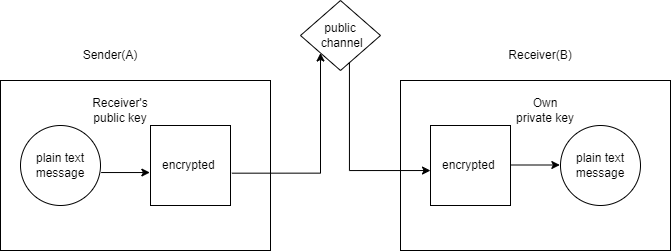
\includegraphics{public.png}
%      \caption{Caption}
%      \label{fig:my_label}
%  \end{figure}

  \chapter{Diffie - Hellman Key Exchange}
        We need some mathematical foundations to understand the Diffie - Hellman Key Exchange.
   \section{Mathematical Foundations}
             \begin{itemize}
			    \item \textbf{Definition}\\
			    A \textbf{prime number} is a natural number greater than 1 that has no positive integer divisors other than 1 and itself.\\
			    \vspace{3mm}
			   \textit{Example:-} 2, 3, 5, 7, 11 etc.\\
			     
			     \item \textbf{Definition}\\
			    Two positive integers are said to be \textbf{relatively prime} (or \textbf{ co prime}), if their greatest common divisor (GCD) is 1.\\
			    \vspace{3mm}
                 \textit{Example:-} 5 and 7
               \item \textbf{Definition}\\
                 For a positive integer $n$, the integers $a$ and $b$ are \textbf{congruent} modulo $p$, if their remainders when divided by $p$ are same.
                 $$ a \equiv b \;(\text{mod} p) \iff a \mod p = b \mod p $$ 
                
                 \textit{Example:-}
                  $52 \equiv 24 \;(\text{mod} 7)$\\
          \item \textbf{Definition}\\
                 A  number $g$ is called a \textbf{primitive root} (or \textbf{a generator}) modulo $p$ if every integer relatively prime to $p$ is congruent to a power of $ g \mod p$.\\
                 \vspace{2mm}
                   If we take a set $\{1,...p-1\}$ which is equal to the set $ \{g^1,g^2 ...g^p^-^1 \} \;(\text{mod} p)$ .\\
                 \vspace{3mm}
			    \textit{Example:-} 2 is a primitive root of prime number 5 \\
       \end{itemize}
  
            \begin{itemize}
               \item \textbf{Definition}\\
               A \textbf{safe prime} is a prime number $p$ of the form $p=2q+1$ where $q$ is also a prime number. \\
               In such a case $q$ is called a \textbf{sophie germain prime}\cite{Stiglic2005}.\\
               \vspace{5mm}
               \textit{Example:-} 23 is a safe prime, because\\
               $$2*11+1=23$$
               where $11$ is called sophie germain prime.
			    \item \textbf{Definition}\\
			    Let $g$ be a primitive root of prime number $p$, and for any $a\in \{1,2,....p-1\}$ there exist $x \in \{1,...p-1\} $ such that 
			    $$ g^x = a \;(\text{mod} p)$$\\
			    It can be written as, $$x = \log_g a \;(\text{mod} p)$$\\
			    We consider $x$ as unique and the problem of finding $x$ is called as the \textbf{discrete logarithm problem}.\\
			    \vspace{2mm}
			    \textit{Example:-} $2^9 = 6(mod 11) \implies \log_2 6= 9 \;(\text{mod} 11)$
			  
            \end{itemize}
 
\section{Key Establishment}

        \begin{quote}
           "If you look right under the center of a streetlight, you don't find anything that wasn't known before.
	  	   If you look out into the darkness, you don't discover anything, cause you can't see anything. 
		    So you're always working at the edge of the streetlight, trying to find your keys."
		          - Whitfield Diffie \cite{stamp2007applied}
 \end{quote}  

    \begin{itemize}
     Let $p$ be a large prime and g is an integer where $2\leq g\leq p-2$.
    	Both the prime $p$ and generator $g$ are publicly known.\\
    	\vspace{2mm}
    	\textbf{step 1:-} Alice chooses a random number $a$, where $1\leq a \leq p-2$ and calculates $\alpha = g^a \;(\text{mod} p)$.\\
    	\vspace{2mm}
        \textbf{step 2:-} She then sends $\alpha$ to Bob. \\
    	\vspace{2mm}
    	\textbf{step 3:-} Bob also chooses a random number b, where $1\leq b \leq p-2$ and calculates $\beta = g^b \;(\text{mod} p)$ and then sends $\beta$ to Alice. \\

	 \textbf{step 4:-} Alice then calculates
	  \vspace{2mm}
	  $$\beta^a \;(\text{mod} p) = (g^b)^a \;(\text{mod} p) = g^a^b \;(\text{mod} p)$$ \\
	  \vspace{2mm}
	 \textbf{step 5:-} and Bob computes 
	  \vspace{2mm}
	  $$\alpha^b \;(\text{mod} p) = (g^a)^b \;(\text{mod} p) = g^a^b \;(\text{mod} p)$$\\
	  \vspace{2mm} \\
	  \textbf{step 6:-} Alice and Bob now share $g^a^b \;(\text{mod} p)$, which can be used as a \textbf{Symmetric key}\cite{stamp2007applied}.\\
     
        \textbf{Remarks}\\
	   \item The security of the Diffie-Hellman key Exchange depends on the computation complexity of tackling the \textbf{discrete logarithm problem}.
	   \item There's no effective calculation to fathom the discrete logarithm problem
	   \item The security of many cryptosystems is based on DLP.\\
	    	\end{itemize}
	    	
      Using any of the exponential algorithms it is infeasible for large primes.
       However, for large $p$, an exhaustive search is not feasible. 
         Some of the current discrete log algorithms are
         \begin{itemize}
         \item Trivial Multiplication
         \item Baby-step Giant-step Algorithm
          \end{itemize}
           \textbf{Advantages}
    \begin{enumerate}
        \item Once the key exchanged, the communication of data can be done through insecure channel.
        \item the sharing of the secret key is safe.
        \item The sender and receiver do need prior knowledge of each other.
     \end{enumerate}
     
     \text Example program will be shown in Python and in Sage.
     
     \chapter{Man-in-the-Middle Attack}
     \begin{itemize}
			        \item The Diffie-Hellman key Exchange is subject to man-in-the-middle attack, in the event that there's no strategy to verify the members amid the key Exchange.\\
			        \item If the attacker (Trudy) wants to see the messages that are being sent between Alice and Bob,\\
			        she can interrupt the process in the following way.
			    \end{itemize}
		
   \begin{enumerate}
           \item Trudy chooses an exponent t. \\
           \item She then intercepts $g^a (\mod p)$ and $g^b (\mod{p})$ and sends $g^t (\mod {p})$ to Alice and Bob.\\
           \item At this point, Alice believes $g^t(\mod{p})$ came from Alice.\\
           \item Now Trudy computes $K_A = (g^a)^t (\mod {p})$ and $K_B = (g^b)^t (\mod {p}$
           \item Alice computes $K_A$ and Bob computes $K_B$
           \item Then when Alice sends a message to Bob (encrypted with $K_A$), Trudy can intercept it, decrypt it and re-encrypt it (or encrypt a different message) with $K_B$ before sending it on to Bob. 
       \end{enumerate}
       
      \text Example program will be shown in Python. 
      
       \chapter{Diffie - Hellman Key Exchange conclusion}
       \begin{itemize}
       \item  The Diffie-Hellman key exchange is one of the most useful and widely used public key cryptosystems.\\
       \item It provides elegant solution to the so-called \textit{key establishment problem} (or key distribution problem), that is, how to securely agree on a shared symmetric key.\\
       \item  Care must be taken when using Diffie-Hellman, since the man-in-the-Middle attack is a serious threat. But it can be prevented in many important applications.\\
       \item Diffie-Hellman is used in the IPSec protocol to provide \textit{perfect forward secrecy} (PFS).\\
    
           \item \textit{Perfect forward secrecy(PFS)} alludes to an encryption system that changes the keys utilized to encrypt and decrypt information frequently and automatically.
           \item Using Ephemeral Diffie-Hellman, we can achieve perfect forward secrecy (PFS)
           \item In Ephemeral Diffie-Hellman a temporary key is generated for every connection.
       \end{itemize}
       \chapter{Arithmetica Key Exchange}
	    \section{Mathematical Foundations}
		    \item \textbf{Definition}:-\\
		    A \textbf{Group} $<G,*>$ is a non-empty set G, together with a binary operation $*$ on G, which satisfies following axioms.\\
		        \item \textbf{Associativity}:-
		    \begin{itemize}
		        \item The binary operation * is associative, if 
		        $$(a*b)*c = a*(b*c), \forall a,b,c \in G$$.
		    \end{itemize}
		    \item \textbf{Identity}:-
		    \begin{itemize}
		        \item For any element there exists the identity that is for all $a\in G$ such that\\
		        $$e*a = a*e = a$$
		        \end{itemize}
		        \item \textbf{Inverse:-}
             \begin{itemize}
		            \item For each element $a \in G$, there exists an element $a^-^1 \in G$ such that\\
		            $$a^-^1*a = a*a^-^1 = e$$.
		            \end{itemize}
		            \item \textbf{Closure:-}
		            \begin{itemize}
		                \item The group is closed under the operation, if any two elements\\
		                a and b are in G, then $a* b$ is also in G  that is for any $a,b \in G$.\\
		                $$(a*b)\in G$$.
		            \end{itemize}
		            \textbf{Definition}\\
        A group $<G,*>$ is \textbf{"an abelian (or a commutative)"} if it satisfies,
        $$a*b = b*a, \forall a,b\in G.$$\\
        \textbf{Definition}\\
       A \textbf{conjugacy class} of a group is a set of elements that are connected by an operation called \textbf{conjugation}.\\
       \vspace{2mm}
    An element 'b' in a group G is \textbf{conjugate} to an element 'a' if there exists a $g\in G$ such that $$a = gbg^{-1}, \forall a,b \in G$$ \\
    Alternatively, one says that a is a \textbf{conjugate} of b.
    \textbf{Properties}\\
    There are three properties for conjugacy class\\
    \vspace{2mm}
    \textbf{Reflexivity}\\
    \begin{itemize}
        \item If a is conjugate to a then it follows that\\
    $$a=eae^{-1}$$\\ where e is the identity element of the group.
    \end{itemize}
    
     \textbf{Symmetry}\\
    \begin{itemize}
        \item If a being conjugate to b implies b being conjugate to a.\\
        This follows from 
        $$ a=gbg^{-1} \implies b=g^{-1}a(g^{-1})^{-1}=g^{-1}ag .$$
    \end{itemize}
    \textbf{Transitivity}\\
    \begin{itemize}
        \item that a being conjugate to b and b being conjugate to c implies that a is conjugate to c. \\
        This follows from \\
        $$a=gbg^{-1}, b=gcg^{-1} \implies a=gcg^{-1} .$$
     \end{itemize}
     \textbf{Definion}\\
     A group $<G,*>$ is \textbf{"free group"} if there exists no relation between its group generators other than the relation between an element and its inverse.\\
     \vspace{2mm}
    \textit{Example:-} Consider the set G of finite words\\
    $\{1_G,a,b,a^-^1,b^-^1\}$ where $1_G$ is empty word of G.\\

    Typical elements of G include
     $$abaab^-^1b^-^1, bba^-^1a1_Gba,bbbb,aba^-^1b^-^1,a,b^-^1,1_G$$
     \textbf{Remark}\\
     The order of the elements matter, which means '$ab$' and '$ba$' are two different words in G.\\ 
     Then G is called '\textbf{non-abelian group}'.\\
     \vspace{3mm}
     A \textbf{binary operation} $*$ can be defined on G,\\
     $$aba^2b^-^2*b^3a=aba^2b^-^2b^3a=aba^2ba$$.
     
     \textbf{Idea}\\
      \begin{block}
       We present a compact algebraic key establishment protocol, using group-theoretic illustration.
       For secret key establishment between two individuals whose only means of communication is a \textbf{public channel}.
     The protocol requires each party to perform an algebraic computation ( several multiplications like rewriting groups).
      The result of the computation are then exchanged
      And a common shared secret key is then obtained after a few calculations. 
      \end{block}
    
     \section{Key Establishment }
     \vspace{2mm}
     \textbf{step 1:-} A finitely presented, infinite non-abelian group G is made public.\\
    \textbf{step 2:-} Alice and Bob create their    public keys to be subgroups of G, say
    $$S_A=<s_0,s_1,...s_{n-1}>$$ and $$  S_B=<t_0,t_1,...t_{m-1}>$$
    \textbf{step 3:-} $S_A$ and $S_B $ can be     considered as a set of words $s_i$ and $t_j$  respectively, with the binary operation of    concatenation subject to the relations of G.
    \textbf{step 4:-} Alice and Bob select their private keys,\\
      
      $$a=s^{i_0}_{\sigma(0)}...s^{i_{n-1}}_{\sigma(n-1)} \in S_A$$ and
      
      $$b=t^{j_0}_{\tau(0)}...t^{j_{m-1}}_{\tau(n-1)} \in S_B.$$
       \textbf{step 5:-} Then Alice computes set of elements like concatenating with Bob's public key \\
      $$\{a^{-1}t_{0}a,....a^{-1}t_{m-1}a\}$$ 
      and sends result to Bob.\\
      \textbf{step 6:-} Bob computes \\
      $$\{b^{-1}s_0b,...,b^{-1}s_{n-1}b\}$$
      and sends result to Alice.
      \textbf{Conjugation of data}\\
      Before transmission, each of these sets rewritten to obscure private keys a and b.\\
     \begin{itemize}
         \item  With the information received from Bob, Alice is able to compute $b^{-1}ab$ since\\
      $$b^-1ab=b^{-1}s^{i_0}_{\sigma(0)}....s^{i_{n-1}}_{\sigma(n-1)}b$$\\
              $$=b^{-1}s^{i_0}_{\sigma(0)}bb^{-1}....b^{-1}s^{i_{n-1}}_{\sigma(n-1)}b$$\\
              $$=(b^{-1}s_{\sigma(0)}b)^{i_0}...(b^{-1}s^{i_{n-1}}_{\sigma(n-1)})^{i_{n-1}}$$
     \end{itemize}
     \begin{itemize}
          \item Similarly, Bob computes $a^{-1}ba$ \\
          $$a^{-1}ba=a^{-1}t^{j_0}_{\tau(0)}a...a^{-1}t^{j_{m-1}}_{\tau(m-1)a}$$\\
          $$=a^{-1}t^{j_0}_{\tau(0)}aa^{-1}t^{j_1}_{\tau(1)}a....a^{-1}t^{j_{m-1}}_{\tau(m-1)}a$$\\
          $$=(a^{-1}t_{\tau(0)}a)^{j_0}...(a^{-1}t_{\tau(m-1)}a)^{j_{m-1}}$$
      \end{itemize}
      \textbf{step 7:-} Alice and Bob each compute \\
     $a^{-1}b^{-1}ab$, this can be served as \textbf{shared symmetric key}\cite{stamp2007applied}.
     \pagebreak
     \section{Example}
     
     \begin{itemize}
          \item Alice and Bob select a group,\\
          $$G=<x,y|x^4,y^2,yxyx>$$
          which is public.
          \item Alice's public key $\implies$\\
          $$S_A=<s_0,s_1>=<x^2,y>=\{1_G,x^2,y,x^2y\}$$
          \item Bob's public key $\implies$\\
          $$S_B=<t_0>=<x>=\{1_G,x,x^2,x^3\}$$
        \end{itemize}
        \begin{itemize}
         \item Alice's random private key $\implies$\\
         $$a=(x^2)^2(y)^{-1}=x^4y^{-1}=1_Gy^{-1}=y^-1$$
         \item Bob's random private key $\implies$\\
         $$b=(x)^3=x^3$$
       \end{itemize}
       
       \begin{itemize}
          \item Alice computes $$a^{-1}t_0a=y^{-1}xy$$ and \textbf{rewrites} as $\{yxy\}$.
          \item She then sends $\{yxy\}$ to Bob
          \vspace{3mm}
          \item Bob also computes and rewrites
          $$b^{-1}s_0b=x^{-3}x^2x^3=x^2=x^{-2}$$ and
          $$b^{-1}s_1b=x^{-3}yx^3=xyx^3=x x^{-3}y=x^{-2}y=x^2y$$
          \item He then sends  $\{x^{-2},x^2y\}$ to Alice.
      \end{itemize}
      \begin{itemize}
          \item To establish a common key, Alice computes \\
          $$b^{-1}ab=(x^{-2})^2(x^2y)^{-1}$$
          $$=x^4y^{-1}x^{-2}$$
          $$=1_Gy^{-1}x^{-2}$$ 
          $$=yx^2$$
          $$=x^2y$$
      \end{itemize}
       \begin{itemize}
       \item Finally Alice computes 
         $$a^{-1}(b^{-1}ab)=(y^{-1})^{-1}(x^2y)=yx^2y$$
         $$=x^2$$ This is a symmetric key.\\
         \item similarly, Bob computes
         $$a^{-1}ba=(yxy)^3=yxy\cdot yxy \cdot yxy$$
         $$=yxy^2xy^2xy^2xy$$
         $$=yx1_Gx1_Gxy $$
         $$yx^3y$$
         $$=x$$
     \end{itemize}
     \begin{itemize}
          \item Bob then computes\\
          $$a^{-1}b^{-1}a=(a^{-1}ba)^{-1}=x^{-1}$$
          Using above value he calculates shared secret.\\
          $$(a^{-1}b^{-1}a)b=x^{-1}x^3$$
          $$=x^2.$$
          Alice and Bob can then compute a shared symmetric key based on this shared secret.
      \end{itemize}
      \begin{itemize}
          \item  The security of Arithmetica is based on the computational complexity of the \textbf{conjugacy problem}
          \item We can recover the private keys a and b from the group, \\
          using \textbf{canonical form}\cite{stamp2007applied}. 
      \end{itemize}
    			    
\chapter{Hughes-Tunnenbaum Length Attack}
			    \item The basic idea to of the attack on Arithmetica is that group elements with long lengths.\\
			     What is a canonical form?\\
			     For any element $w \in G$, the \textbf{length} of w to be\\
			        $$l(w)=|k_0|+|k_1|+...+|k_{N-1}|,$$
			        where $$w=g^{k_0}_{i_0}g^{k_1}_{i_1}...g^{k_{N-1}}_{i_{N-1}}$$
	     	
           For any two words $x,y \in G$, we see that the lengths satisfy\\
           $$l(xy)\leq l(x)+l(y).$$
           If some of the parts of x and y cancel,then it may be that the length of xy is much shorter than the sum of the lengths of x and y. 
            As above, let\\
           $$a \in S_A = <s_0,s_1,....s_{n-1}>$$ be Alice's private key.
           
         First, we assume that the factors $s_i$ have lengths which are large, relative to the length of a. 
         From Bob's public key,\\
          $$S_B=<t_0,t_1,...t_{m-1}>,$$
          Alice computes $u_r = a^{-1}t_ra$, for $r=0,1,...,m-1$, and sends these to Bob.
          The attacker Trudy performs the length attack by repeatedly computing\\
         $$l(s^{\pm 1}(u_r)s^{\pm 1}_i).$$
        
            If she finds that\\
           $$l(s^{\pm 1}_i(u_r)s^{\pm 1}-i < l(u_r),$$
          Trudy concludes that $s^{\pm 1}_i$ is a factor of a on the left- not with certainity but with some positive probability. 
           \vspace{3mm}
        Once a factor is recovered, the attack is similarly applied again to recover another factor of a and this process is repeated to recover all of a, with some positive probability. 
         
            The length attack is effective when the $l(s_i)$ are large. 
           \item If the length of each element is less  than ten the attack can be prevented.
        
         \chapter{Arithmetica Key Exchange conclusion}
			\begin{itemize}
			    \item Arithmetica uses very sophisticated mathematics
			    \item In the world of public cryptography, where advanced mathematics plays a significant role in the design and analysis of cryptosystems. 
			    \item In elliptic curve cryptography, group-based cryptosystems and lattice-based encryption schemes illustrate this point \cite{stamp2007applied}.
			\end{itemize}
  
    	\bibliographystyle{plain}
    	\bibliography{Bibiliography}

\end{document}